After training the model with the Icons-50 dataset for 100 epochs, I was able to achieve a remarkable classification accuracy on the discriminator, seen in Fig.~\ref{fig:Icons50Acc} , with a 94\% accuracy for real images and a 98\% accuracy for generated images.

\begin{figure}[htbp]
    \centering
    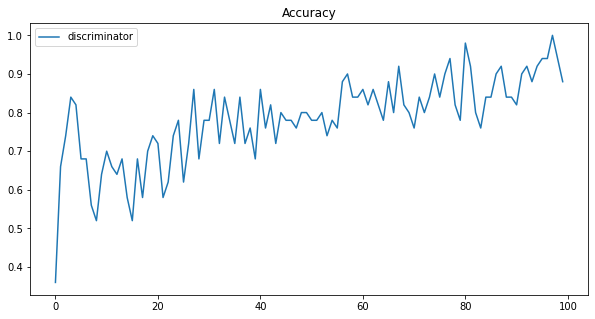
\includegraphics[width=0.48\textwidth]{images/icons50/icons50_acc}
    \caption{Discriminator accuracy on the Icons-50 dataset}
    \label{fig:Icons50Acc}
\end{figure}

In terms of loss, while the discriminator finished with a satisfactory minimal loss of 0.329, the same could not be said for the generator, as its loss kept increasing as the training went along, finishing at a value of around 2.532, as can be seen in Fig.~\ref{fig:Icons50Loss} .

\begin{figure}[htbp]
    \centering
    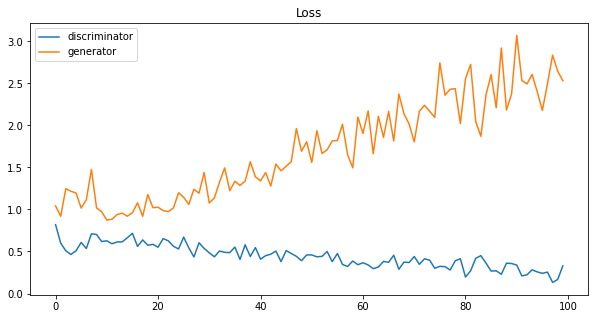
\includegraphics[width=0.48\textwidth]{images/icons50/icons50_loss}
    \caption{Model loss on the Icons-50 dataset}
    \label{fig:Icons50Loss}
\end{figure}

Afterwards, I trained a new model, with the same structure, on the Icons-10 subset, again for 100 epochs.
When analyzing the discriminator's performance, it seemed that both its loss and accuracy suffered.

While the loss only increased slightly, to an acceptable value of 0.643, the accuracy while classifying images as real or fake varied quite drastically during training, as can be seen on Fig.~\ref{fig:Icons10Acc} , finishing at, respectively, 83.33\% and 86.67\%.

\begin{figure}[htbp]
    \centering
    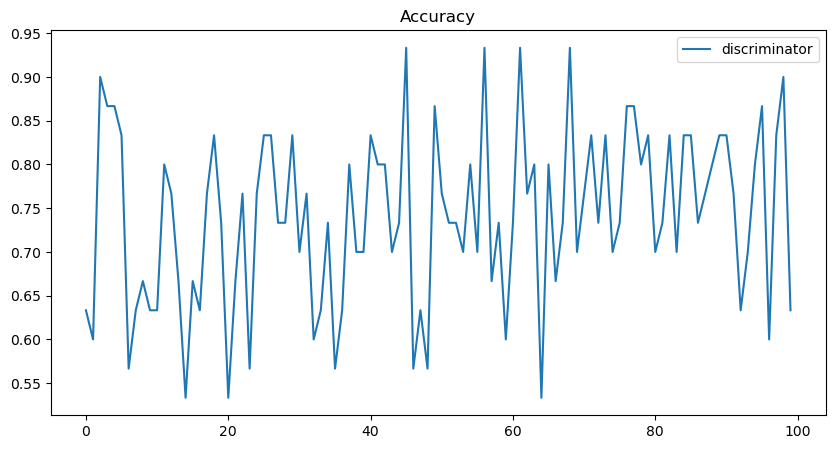
\includegraphics[width=0.48\textwidth]{images/icons10/icons10_acc}
    \caption{Discriminator accuracy on the Icons-10 dataset}
    \label{fig:Icons10Acc}
\end{figure}

In terms of the generator's performance, while the loss still varied quite significantly, the new dataset proved successful, with the model finishing with a much better loss of 1.433, as seen on Fig.~\ref{fig:Icons10Loss} .

\begin{figure}[htbp]
    \centering
    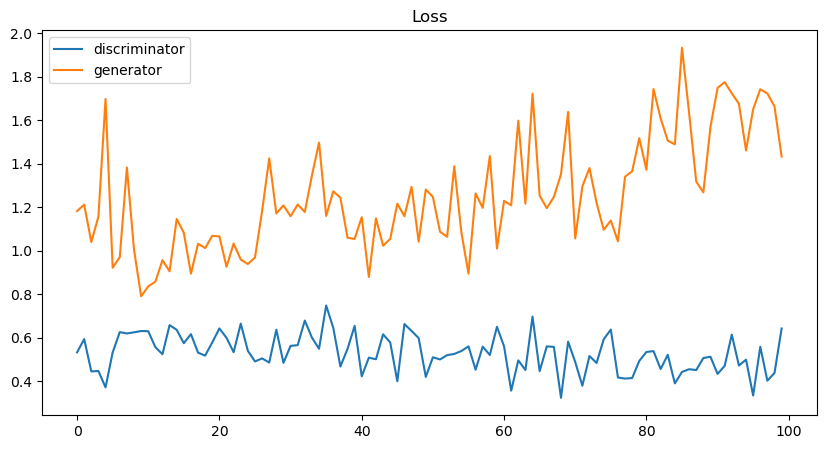
\includegraphics[width=0.48\textwidth]{images/icons10/icons10_loss}
    \caption{Model loss on the Icons-10 dataset}
    \label{fig:Icons10Loss}
\end{figure}

To better evaluate the performance of the trained generators, I generated a new set of icons belonging to the classes common to both datasets.

When given a simple task, such as generating a ``clock'' icon, the model trained on the Icons-50 dataset only seemed to perceive the shape of the clock, with none of the defining details being present in the generated images, evident from Fig.~\ref{fig:Icons50Clock}.

The second model performed much better on this task, capturing finer details such as the correct color, and the hour and minutes hands, as it is clear from Fig.~\ref{fig:Icons10Clock}.

\begin{figure}[htbp]
    \begin{subfigure}[h]{0.4\linewidth}
        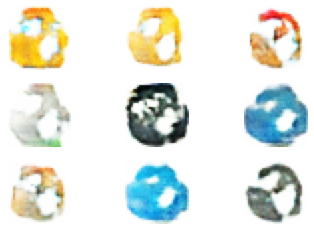
\includegraphics[width=\linewidth]{images/gen_icons/icons50_clock}
        \caption{Icons-50 dataset}
        \label{fig:Icons50Clock}
    \end{subfigure}
    \hfill
    \begin{subfigure}[h]{0.4\linewidth}
        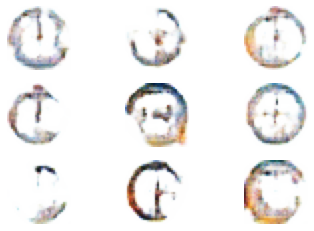
\includegraphics[width=\linewidth]{images/gen_icons/icons10_clock}
        \caption{Icons-10 dataset}
        \label{fig:Icons10Clock}
    \end{subfigure}
    \caption{Generated icons belonging to class ``clock"}
\end{figure}

When dealing with a complex task, such as generating icons for the ``family'' class, the original generator was able to create recognizable images, even though they lacked definition and variability, as seen on Fig.~\ref{fig:Icons50Family}.

When trained on the Icons-10 dataset, the model was able to generate a unique and slightly more detailed set of icons, albeit with variable results, as seen on Fig.~\ref{fig:Icons10Family}.

\begin{figure}[htbp]
    \begin{subfigure}[h]{0.4\linewidth}
        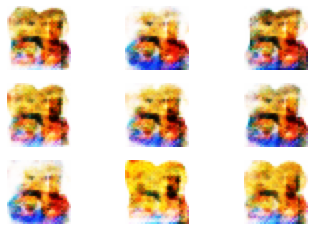
\includegraphics[width=\linewidth]{images/gen_icons/icons50_family}
        \caption{Icons-50 dataset}
        \label{fig:Icons50Family}
    \end{subfigure}
    \hfill
    \begin{subfigure}[h]{0.4\linewidth}
        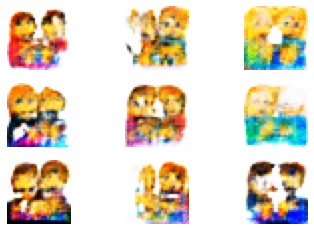
\includegraphics[width=\linewidth]{images/gen_icons/icons10_family}
        \caption{Icons-10 dataset}
        \label{fig:Icons10Family}
    \end{subfigure}
    \caption{Generated icons belonging to class ``family"}
\end{figure}